\chapter{Multi-task learning}

So far we have considered \ac{AES} and \ac{NLI} as independent tasks and
performed experiments on both tasks separately. We will now try to train
models to predict both tasks simultaneously.


\section{Models}

We selected four models for the multi-task experiments, two convolutional and
two recurrent neural networks. They were chosen based on the macro \FI results
on the development set. The two \acp{CNN} chosen were the two \acp{CNN} that
had the highest macro \FI on the full set of labels in the development set,
and likewise for the two \acp{RNN}. The hyperparameters for the four models are
summarized in tables \ref{tab:cnn-parameters} and \ref{tab:rnn-parameters}.

\begin{table}
  \centering
  \begin{tabular}{lll}
    \toprule
    Hyperparameter & CNN1 & CNN2 \\
    \midrule
    Word embeddings & \multicolumn{2}{c}{Dynamic} \\
    Embedding size & \multicolumn{2}{c}{100} \\
    $L_2$ constraint & \multicolumn{2}{c}{3} \\
    Windows & \multicolumn{2}{c}{3,4,5} \\
    Embedding init & Random & Pre-trained \\
    Input representation & Mixed UPOS & Tokens \\
    \bottomrule
  \end{tabular}
  \caption{Descriptions of the two CNN models}
  \label{tab:cnn-parameters}
\end{table}

\begin{table}
  \centering
  \begin{tabular}{lll}
    \toprule
    Hyperparameter & RNN1 & RNN2 \\
    \midrule
    Word embeddings & \multicolumn{2}{c}{Dynamic} \\
    Embedding size & \multicolumn{2}{c}{100} \\
    RNN cell & \multicolumn{2}{c}{GRU} \\
    Pooling method & \multicolumn{2}{c}{Attention} \\
    Bidirectional & \multicolumn{2}{c}{Yes} \\
    Embedding init & Random & Pre-trained \\
    Input representation & Tokens+UPOS & Tokens \\
    \bottomrule
  \end{tabular}
  \caption{Descriptions of the two RNN models}
  \label{tab:rnn-parameters}
\end{table}

The multi-task models have two outputs with different loss functions. The
CEFR output is a single regression node with sigmoid output and mean squared
error loss. The NLI output is a softmax layer with seven nodes, and uses
categorical cross-entropy loss. To train the models, they are optimized to
minimize the sum of losses for both output layers. We multiply each loss by a
weight before summing to see how performance is influenced by which loss has
most weight. We ensure that the sum of weights is equal to 1. An auxiliary
loss weight of $0.5$ thus means that both losses have equal weight. An
auxiliary loss weight of $0.2$ means that the loss on the main task has
weight $0.8$.

We chose ten different auxiliary loss weights, and for each loss weight we
trained and evaluated each model five times with different random seeds. By
training more than one model with a given set of hyperparameters, we can get
an idea of the variance of results.

We know that the sigmoid output used for regression on the main task yields
values between 0 and 1, and that the target value is also between 0 and 1.
Therefore, the prediction error is also bounded between 0 and 1. We are using
squared error loss, and squaring a number between 0 and 1 gives a smaller
number. However, the cross-entropy loss on the auxiliary output is always a
number bigger than 0, but unbounded from above. This suggests that a small
auxiliary loss weight may be preferable, so the loss from our main task is
not drowned in the loss from the auxiliary task.


\section{Results}

The reported metrics apply to the main task, CEFR prediction, only.

The highest macro \FI scores on the full label set all come from RNN models.
Three of them was achieved by RNN2 and two by RNN1. The five highest scores
range between $0.468$ and $0.483$ and were achieved using auxiliary loss
weights in the range from $0$ to $0.5$. The highest score was achieved in
single-task mode, but with a different random seed than before. The highest
macro \FI score in the previous chapter was $0.460$.

On the set of collapsed labels, the five highest macro \FI scores range
between $0.798$ and $0.824$. Four of the top five results are from RNN1, and
one from RNN2. Here, the auxiliary loss weights range from $0$ to $0.2$. The
two highest scores were also achieved in single-task mode with a different
random seed than before. Additionally, the model that had the highest macro
\FI score ($0.806$) on the collapsed set of labels in the previous chapter
was not included in the multi-task experiments. RNN1 and RNN2 had respective
macro \FI scores of $0.687$ and $0.773$ on the collapsed set of labels in the
previous chapter.

Below we plot the effect of auxiliary loss on all four models (fig.
\ref{fig:lossweight}). The $x$ value is the weight given to the auxiliary
loss during training. Some of the models have an auxiliary loss weight of
zero, which is the same as training in single-task mode. The 95\% confidence
intervals indicated by shaded areas in the plots are computed in the plotting
software Seaborn \autocite{seaborn}, using a bootstrap sampling method.

\begin{figure}
  \centering
  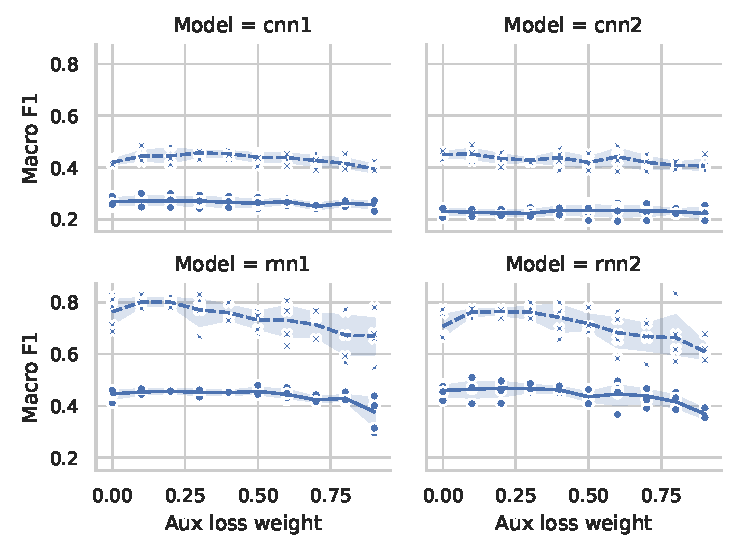
\includegraphics{lossweight}
  \caption[Performance of multi-task models]{
    Lines follow the mean of macro \FI scores. Shaded areas show 95\%
    confidence interval for the mean. Results for the collapsed set of
    classes are plotted with cross symbols and dashed lines.
  }
  \label{fig:lossweight}
\end{figure}

The effect of auxiliary task weight is most visible for the RNN2 model, where
we see a degradation of results as the auxiliary loss weight gets closer to
1. In RNN1, a different effect seems apparent, namely an increase in variance
with increased auxiliary loss weight. The RNN1 experiment that entered the
top five with an auxiliary loss weight of $0.5$ appears from the to be an
outlier. Most of the best results are a result of single-task training or a
low auxiliary loss weight, confirming our suspicions above regarding the
magnitude of loss functions. In model RNN2, it looks like a small auxiliary
loss weight of $0.1$ has reduced the variance in results compared to the
experiments in single-task mode.

For the experiments using collapsed CEFR labels, we see in three of the four
models that the mean macro \FI score (the dashed line in the plot) is highest
using a small auxiliary loss weight of $0.1$. However, the variance is large,
especially in the RNN models.

However, even though we are now running the same experiment multiple times
using different random seeds, we still have only five samples for each
auxiliary loss weight, which is a small number to try to draw any conclusions
from with statistical certainty.

\begin{figure}
  % cnn-multi-26728430_2.pkl
  \begin{subfigure}{\linewidth}
    \centering
    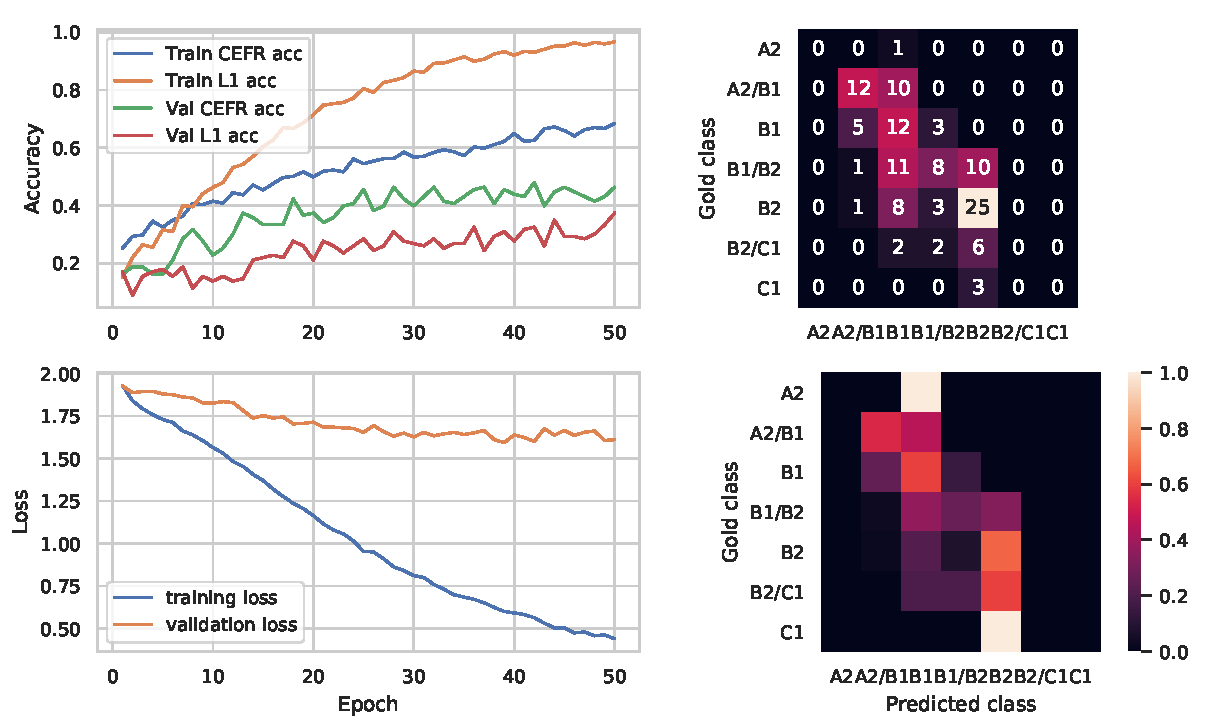
\includegraphics{cnn-multi-training}
    \caption{Training and validation loss and accuracy over 50 epochs of training.}
  \end{subfigure}
  \begin{subfigure}{\linewidth}
    \centering
    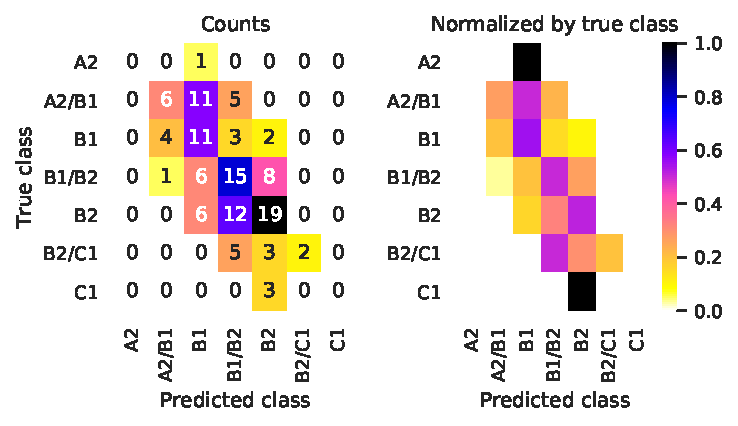
\includegraphics{cnn-multi-confusion}
    \caption{Confusion matrix on validation set, raw counts and normalized.}
  \end{subfigure}
  \caption[Training behaviour of a multi-task CNN]{
    Training behaviour of a CNN1 with an auxiliary loss weight of $0.3$.
    Macro \FI = $0.293$.
  }
  \label{fig:cnn-multi-training}
\end{figure}

\begin{figure}
  % rnn-multi-26728427_18.pkl
  \begin{subfigure}{\linewidth}
    \centering
    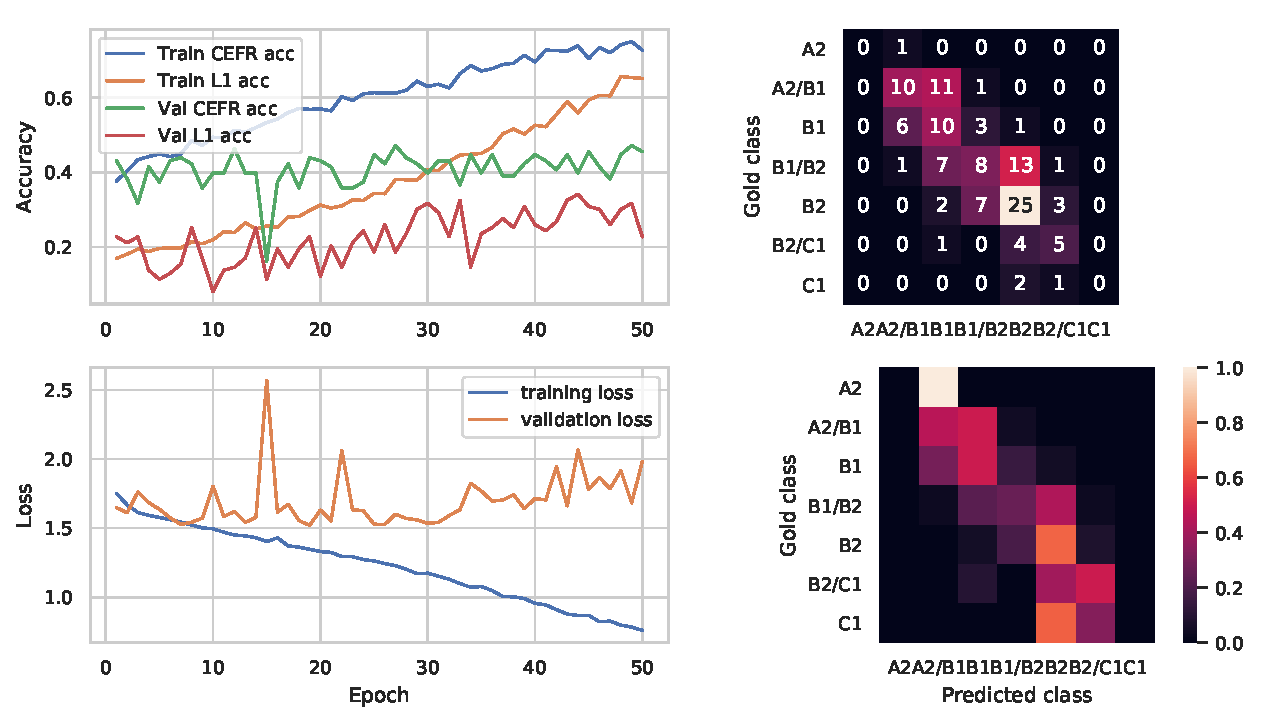
\includegraphics{rnn-multi-training}
    \caption{Training and validation loss and metrics over 50 epochs of training.}
  \end{subfigure}
  \begin{subfigure}{\linewidth}
    \centering
    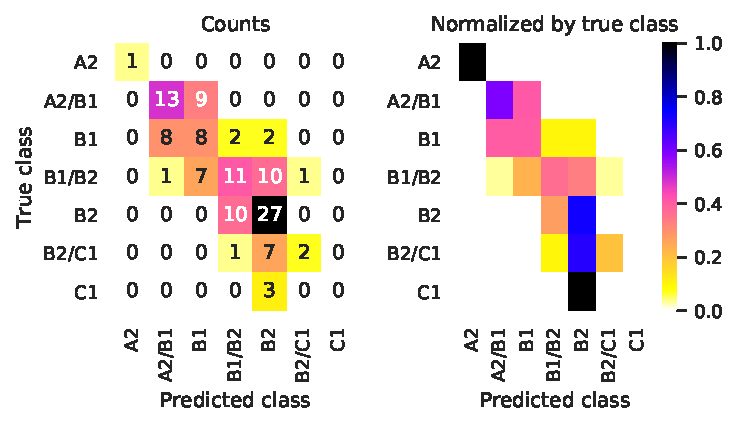
\includegraphics{rnn-multi-confusion}
    \caption{Confusion matrix on validation set, raw counts and normalized.}
  \end{subfigure}
  \caption[Training behaviour of a multi-task RNN]{
    Training behaviour of an RNN1 with an auxiliary loss weight of $0.1$.
    Macro \FI = $0.471$.
  }
  \label{fig:rnn-multi-training}
\end{figure}

In the plots of training behaviour, we see that both the CNN and RNN models are
able to overfit the training data on the \ac{NLI} task. On the \ac{AES} task,
training stops before the training MAE converges, but for both models the
validation metrics seem to have stopped improving long before 50 epochs.

As before, the validation loss for the RNN model has much bigger fluctuations
than the CNN model. The RNN validation loss (figure
\ref{fig:rnn-multi-training}(a), left) seems to have a baseline at around
$0.2$, with fluctuations that occasionally exceed $0.4$ and approach $0.6$.
The CNN validation loss (figure \ref{fig:cnn-multi-training}(a), left) is
quite stable, but around a higher value, somewhere between $0.5$ and $0.6$.


\section{Correlation of metrics}

Even though we decided previously to use macro \FI score as our main
evaluation metric, it is still interesting to compare it to alternative
evaluation methods, especially since there is so much variation in evaluation
metrics used for \ac{AES} in the literature. In particular, we want to see if
there are significant differences in how models would be ranked according to
different metrics. Since we now have trained and evaluated a number of
different models, we can compare and contrast their scores on different
metrics by using the prediction they made.

We chose micro \FI score and \ac{MAE} as the metrics to compare with macro
\FI score. The micro \FI lets us compare the effect of macro vs. micro
averaging scores for different classes. On the other hand, \ac{MAE} is a
metric that has an intuitive interpretation on ordinal labels, such as in our
case. It is also a metric that has been reported in previous literature
\autocite{vajjala17}.

\begin{figure}
  \centering
  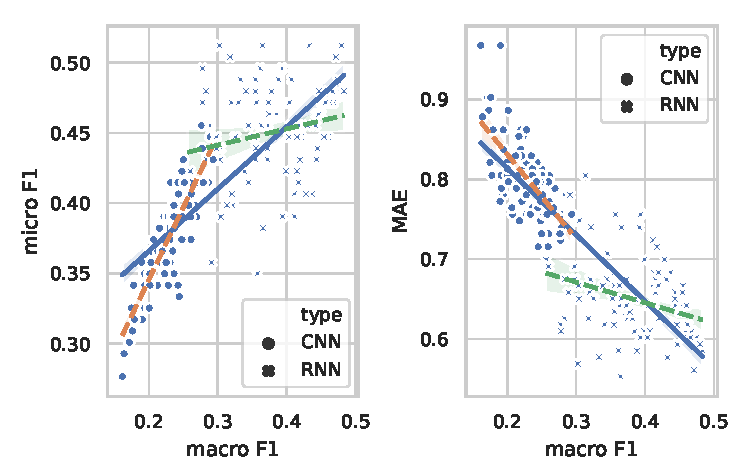
\includegraphics{reg_macro_F1_all}
  \caption[Macro \FI versus MAE]{
    Macro \FI versus micro \FI and MAE for experiments on the full set of
    CEFR labels. Line of regression included in plot. The shaded area covers
    a 95\% confidence interval for the line of regression. CNN models are
    plotted with dots, RNN models with crosses. Lines of regression for the
    sub-populations are plotted in different colours and with dashed lines.
  }
  \label{fig:reg_macro_F1_all}
\end{figure}

\begin{figure}
  \centering
  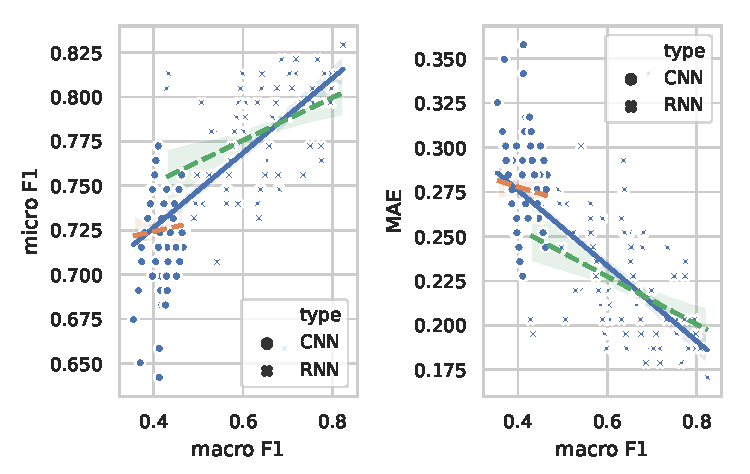
\includegraphics{reg_macro_F1_collapsed}
  \caption[Macro \FI versus micro \FI and MAE]{
    Macro \FI versus micro \FI and MAE for all experiments using collapsed
    CEFR labels. Line of regression included in plot. The shaded area covers
    a 95\% confidence interval for the line of regression. CNN models are
    plotted with dots, RNN models with crosses. Lines of regression for the
    sub-populations are plotted in different colours and with dashed lines.
  }
  \label{fig:reg_macro_F1_collapsed}
\end{figure}

We plotted two pairs of metrics for all experiments in this chapter against
each other. The first pair is macro \FI score against the micro \FI score,
and the second pair is the macro \FI score against the mean average error.
The experiments on the full set of classes and the collapsed set of classes
are separated into two plots, figures \ref{fig:reg_macro_F1_all} and
\ref{fig:reg_macro_F1_collapsed}. From examining the plots, it appears that
the correlation is not all that strong, at least not for macro \FI vs. micro
\FI. Four of the experiments on the full set of classes are tied for the
highest micro \FI, but they range between $0.302$ and $0.480$ in macro \FI.

An interesting effect is that when we use fewer target labels, the mean
absolute error is almost perfectly correlated with the micro \FI. This is
apparent from the plot, since the right-hand plot in figure
\ref{fig:reg_macro_F1_collapsed} is almost a perfect mirror image of the
left-hand plot, flipped top to bottom. We can also quantify this using a
correlation coefficient. For the full set of labels, Pearson's r between
micro \FI and MAE is $-0.913$ ($p < 10^{-78}$). For the collapsed set of
labels, it is $-0.994$ ($p < 10^{-193}$). 

We notice that the CNN and RNN experiments appear to form two separate
populations in the plots, with different correlation properties. In fact, we
see that in almost all cases, the lines of regression for the separate
populations have different slopes from the line of regression for the
combined populations. On the other hand, if there were a linear relationship
between the metrics that was consistent across all populations, we would
expect the regression lines for the sub-populations to be more or less
collinear with the regression line for the combined populations.
\footnote{Two populations can have equal correlation coefficients, but this
does not mean that the lines of regression have equal slope.}

The actual values of Pearson's correlation coefficient for the different
populations and pairs of metrics are tabulated in table
\ref{tab:metric-corrs}. We see that in several cases, the correlation value
is much lower when examining CNN experiments and RNN experiments as separate
populations than when we combine them. The correlation values can be
misleading when we combine two distinct populations into one dataset, since
Pearson's correlation coefficient implicitly assumes that the relationship is
linear. This does not seem to be the case for our data, as indicated by the
different slopes of the regression lines we saw above.

\begin{table}
  \centering
  \begin{tabular}{lrrrr}
    \toprule
             & \multicolumn{2}{c}{Macro \FI vs. micro \FI}
             & \multicolumn{2}{c}{Macro F1 vs. MAE} \\
    \cmidrule(lr){2-3}
    \cmidrule(lr){4-5}
    Experiments & Correlation & $p$-value            & Correlation & $p$-value \\
    \midrule
      & \multicolumn{4}{c}{All CEFR labels} \\
    \midrule
    CNN         & $0.856$     & $7.02\cdot 10^{-30}$ & $-0.670$    & $2.36\cdot 10^{-14}$ \\
    RNN         & $0.196$     & $5.02\cdot 10^{-2}$  & $-0.311$    & $1.65\cdot 10^{-3}$ \\
    CNN+RNN     & $0.775$     & $2.39\cdot 10^{-41}$ & $-0.842$    & $4.39\cdot 10^{-55}$ \\
    \midrule
      & \multicolumn{4}{c}{Collapsed CEFR labels} \\
    \midrule
    CNN         & $0.055$     & $5.88\cdot 10^{-1}$  & $-0.077$    & $4.47\cdot 10^{-1}$ \\
    RNN         & $0.362$     & $2.15\cdot 10^{-4}$  & $-0.383$    & $8.53\cdot 10^{-5}$ \\
    CNN+RNN     & $0.721$     & $2.15\cdot 10^{-33}$ & $-0.720$    & $3.39\cdot 10^{-33}$ \\
    \bottomrule
  \end{tabular}
  \caption[Correlation of metrics]{
    Pearson's correlation coefficient between two pairs of evaluation metrics
    and different subsets of experiments. Two-tailed $p$-values are included.
  }
  \label{tab:metric-corrs}
\end{table}

The most extreme case of the strength of correlation increasing when the
populations are merged happens with the correlation between macro \FI and
micro \FI for collapsed CEFR labels. The CNN experiments are completely
uncorrelated, and the RNN experiments have a very low correlation coefficient
of $0.362$. Still, when combined, the correlation coefficient becomes
$0.721$, with an extremely low $p$-value.

In the other cases, while not as extreme, the Pearson coefficient is
significantly higher for CNN and RNN experiments together than for CNN and
RNN separately. The one exception is the correlation between macro \FI and
micro \FI for the full set of labels, where the CNN group has a higher
correlation coefficient on its own than when combined with the RNN
experiments. Notice also that in this case, the RNN experiments show no
correlation within their group.

A possible interpretation of the high correlation we see in the combined
experiments is that it is not so much an indication of a linear relationship
between the metrics, but merely tells us that one of the two populations
tends to have improved values for both metrics compared to the other
population.

None of the correlations in table \ref{tab:metric-corrs} are as high as the
correlation we observed between micro \FI and \ac{MAE}. This is probably
because the averaging method in macro \FI means that the metric changes in a
different way depending on input, an effect that probably gets even more
noticeable because of the small size of the dataset and the uneven
distribution of target labels.

The $p$-values reported for the correlation are to be taken with a grain of
salt. They were computed with the SciPy library \autocite{scipy}, which
states in its documentation that the $p$-values should be reasonable
for datasets with at least 500 samples. The values in table
\ref{tab:metric-corrs} were computed on samples with either 100 or 200
samples, well below 500.


\section{NLI results with multi-task models}

In this section, we will examine how the models trained with \ac{NLI} as an
auxiliary task perform on this task in isolation. We predict this task using
the same models by using only the output from the auxiliary output layer.

When we trained single-task models for \ac{NLI} in section
\ref{sec:nli-experiments}, the best model had a macro \FI score of $0.526$
and a micro \FI score of $0.528$. This was a unidirectional GRU with UPOS as
side input, and mean-over-time pooling. In the same set of experiments, the
RNN2 architecture had a macro \FI of $0.447$ and an accuracy of $0.480$.

\begin{table}
  \centering
  \begin{tabular}{lrrrr}
    \toprule
    Target     & Precision &  Recall & \FI score & Support \\
    \midrule
    English    &    $0.55$ &  $0.67$ &   $0.60$  &      18 \\
    Polish     &    $0.57$ &  $0.43$ &   $0.49$  &      30 \\
    Russian    &    $0.50$ &  $0.18$ &   $0.26$  &      17 \\
    Somali     &    $0.50$ &  $0.38$ &   $0.43$  &       8 \\
    Spanish    &    $0.38$ &  $0.74$ &   $0.50$  &      23 \\
    German     &    $0.43$ &  $0.30$ &   $0.35$  &      10 \\
    Vietnamese &    $0.71$ &  $0.59$ &   $0.65$  &      17 \\
    \midrule
    Macro \FI  &           &         &   $0.451$ & \\
    Micro \FI  &           &         &   $0.472$ & \\
    \bottomrule
  \end{tabular}
  \caption[Per-class NLI results from multi-task model]{
    Results from predicting NLI on the dev set using the multi-task RNN2. The
    table lists precision, recall, \FI score and support for each target
    \ac{L1}.
  }
\end{table}

When we look at the NLI results from an RNN2 trained with multi-tasking, we
see a macro \FI of $0.451$ and a micro \FI of $0.472$. This is almost the
same level of performance. The macro \FI is slightly higher than it was in
single-task mode, and the micro \FI is slightly lower. However, the
performance is still lower than the best single-task \ac{NLI} model that had
a different architecture.

The multi-task model gives results comparable with training in single-task
mode, but a benefit is the economy of parameters. The weights in the final
prediction layer comprise a small fraction of the total number of weights in
the model, but the multi-task model performs two different tasks at once.


\section{Sanity check vocab size}

Previously we made the decision to limit the vocabulary in the models to only
the word forms that appear in the essays in the training set. This made sense
because we are using dynamic word embeddings that are updated during
training, and only the word forms in the training set receive weight updates
during the backward pass.

This does however also mean that we lose one of the advantages of pre-trained
vectors, and fastText in particular, namely the ability to get vector
representations for words not seen in training. Instead, during evaluation,
words that do not appear in the training set are represented by an
`\_\_UNK\_\_' token that is essentially random, since it has received no
weight updates in training.


\section{Conclusion}

todo
